% !TeX root = ../main.tex
\chapter{狭义相对论}\label{chap:special-relativity}

\begin{intro}
    严格意义上,相对论并不属于普通物理学力学(Mechanics)的范畴,但多数高校的物理学力学课程都会包含狭义相对论的内容,并定性地介绍一下广义相对论,这份笔记自然也不例外。

    狭义相对论这一章可以说是大多数人(包括笔者)重塑物理直觉的开始,也是真正接触现代物理学的开始。
    但不用担心,在严格的逻辑推导和时空图的指引下,你一定能理解狭义相对论的核心思想,并且能够熟练地运用它来分析物理问题。
\end{intro}

\section{狭义相对论的基本原理}

\subsection{经典理论的危机}

19 世纪末,物理大厦上空有两朵乌云:
\begin{itemize}
    \item 黑体辐射的「紫外灾难」
    \item 迈克耳孙-莫雷实验的「以太风」结果
\end{itemize}
这两朵乌云预示着经典物理学的危机,最终导致了量子力学和相对论的诞生。
接下来我们将讨论第二朵乌云,也就是迈克耳孙-莫雷实验的结果。

库仑(Coulomb)在 1785 年提出了电荷之间的相互作用力遵循平方反比定律,半个世纪后,麦克斯韦(Maxwell)在 1865 年成功地将电学和磁学统一成了电磁学,建立了麦克斯韦方程组,预言了电磁波的存在。
他发现空间电磁场可以以波的形式传播,当时假想的传播介质被称为「以太」,麦克斯韦方程组预言了电磁波在真空中的传播速度是一个常数,约为 \qty{3e8}{\metre\per\second},这个速度被认为是以太中的光速。
\begin{equation}
    \left(\nabla^2 - \mu \epsilon \frac{\partial^2}{\partial t^2}\right) \bm{E} = 0
\end{equation}
\begin{equation}
    \left(\nabla^2 - \mu \epsilon \frac{\partial^2}{\partial t^2}\right) \bm{B} = 0
\end{equation}
其中,$ \mu $ 和 $ \epsilon $ 分别是真空的磁导率和电容率,$ \bm{E} $ 和 $ \bm{B} $ 分别是电场和磁场。
根据麦克斯韦方程组,电磁波的传播速度 $ c $ 满足
\begin{equation}
    c = \frac{1}{\sqrt{\mu \epsilon}} \approx \qty{3e8}{\metre\per\second}
\end{equation}
与参考系无关(?)这个结果与经典力学的预期相矛盾(在经典力学中,速度是相对的)。

于是,人们假想了一个「静止」的以太参考系(否则,地心说复活,太猎奇了\ldots),麦克斯韦方程组在这个参考系中成立。
而在其他参考系中,电磁波的传播速度应该是 $ \bm{c} \pm \bm{v} $,其中 $ \bm{v} $ 是参考系相对于以太的速度。

为了验证这个假说,迈克耳孙(Michelson)和莫雷(Morley)设计了一个精密的干涉仪,试图测量地球相对于以太的运动速度。
在这里,我简单介绍一下迈克耳孙-莫雷干涉仪的工作原理。

% 迈克耳孙-莫雷干涉仪:在地球系与以太系中的光路示意图
\begin{figure}[htbp]
    \centering
    \begin{subfigure}[b]{0.45\textwidth}
        \centering
        \begin{tikzpicture}[scale=0.8, >=latex]
            % 画反射镜
            \draw[thick] (0,4) -- (6,4) -- (6,0);
            \fill[pattern=north east lines] (0,4) rectangle (6,4.2);
            \fill[pattern=north east lines] (6,0) rectangle (6.2,4);
            \draw[thick] (1,0) -- (3,0);

            % 画分束器
            \draw[thick, dashed] (1,1) -- (3,3);

            % 画光路
            \draw[thick, ->] (0,2) -- (1.7,2);
            \draw[thick, ->] (1.7,2.4) -- (1.7,3.8);
            \draw[thick, ->] (2,3.8) -- (2,2.4);
            \draw[thick, ->] (2.3,2.1) -- (5.8,2.1);
            \draw[thick, ->] (5.8,1.8) -- (2.3,1.8);
            \draw[thick, ->] (2,1.8) -- (2,0.1);
            \draw[thick, ->] (2,1.8) -- (2,0.4);


            % 文字说明
            \node at (2,0) [below] {观察屏};
            \node at (2.6,3) [above right, scale=0.6] {分束器(半透明反射镜)};
            \node at (1.7,3.1) [left] {$l_2$};
            \node at (4,1.8) [below] {$l_1$};

        \end{tikzpicture}
        \caption{地球系}
    \end{subfigure}
    % \hspace{1cm}
    \begin{subfigure}[b]{0.45\textwidth}
        \centering
        \begin{tikzpicture}[scale=0.8, >=latex]
            % 画反射镜
            \draw[thick] (1,4) -- (7,4);
            \fill[pattern=north east lines] (1,4) rectangle (7,4.2);

            % 画光路
            \draw[thick, ->]  (1,2) -- (2,2);
            \draw[thick, ->]  (2,2) -- (4.5,4);
            \draw[thick, ->]  (4.5,4) -- (7,2);

            \draw[thick, dashed] (4.5,4) -- (4.5,2) node[midway, right] {$l_2$};
            \draw[thick, dashed] (2,2) -- (5,2);

            \node at (2,2) [below] {G};
            \node at (7,2) [below] {G'};

            \coordinate (O) at (2,2);
            \coordinate (A) at (4.5,4);
            \coordinate (B) at (3,2);

            \pic [draw, "$\theta$", angle eccentricity=1.4] {angle = B--O--A};

            \draw[thick, ->] (6,5) -- (7,5) node[midway, above] {$\symbf{v}$};
        \end{tikzpicture}
        \caption{以太系}
    \end{subfigure}
    \caption{迈克耳孙-莫雷干涉仪:在地球系与以太系中的光路示意图}
    \label{fig:michelson-morley-interferometer}
\end{figure}


如 \cref{fig:michelson-morley-interferometer} 所示,干涉仪由一个分束器和两个垂直放置的反射镜组成。
光源发出的光束经过分束器被分成两束,分别沿两个垂直方向传播,经过反射镜反射后重新汇合,形成干涉图样。

设地球相对于以太的速度为 $v$,记 $\beta = \frac{v}{c}$。
在以太系中看,光束在 $G$ 处分开,在 $G'$ 处重新汇合。

对于图中水平方向的光束,在地球系中计算其往返时间:
\begin{equation}
    t_1 = \frac{l_1}{c - v} + \frac{l_1}{c + v} = \frac{2 l_1 / c}{1 - \beta^2}
\end{equation}
即光顺着地球运动的方向传播。

另一条垂直方向的光束,在以太系中计算其往返时间:
\begin{equation}
    t_2 = 2 \frac{l_2}{\sin \theta} \frac{1}{c} = \frac{2 l_2 / c}{\sqrt{1 - \beta^2}}
\end{equation}

两束光到达 $G'$ 点的时间差为
\begin{equation}
    \Delta t = t_1 - t_2 = \frac{2 l_1 / c}{1 - \beta^2} - \frac{2 l_2 / c}{\sqrt{1 - \beta^2}}
\end{equation}
相位差为
\begin{equation}
    n = \frac{c \Delta t}{\lambda} = \frac{2 l_1 / \lambda}{1 - \beta^2} - \frac{2 l_2 / \lambda}{\sqrt{1 - \beta^2}}
\end{equation}

而经过1/4年(约91天)后,地球运动方向改变,重新测量相位差,得到
\begin{equation}
    n' = \frac{2 l_2 / \lambda}{1 - \beta^2} - \frac{2 l_1 / \lambda}{\sqrt{1 - \beta^2}}
\end{equation}
即干涉条纹要移动!
但是,迈克耳孙-莫雷实验的结果却是\textbf{没有}观测到任何干涉条纹的移动,这与以太假说的预期完全相反。

\subsection{狭义相对论基本原理}

为了解释迈克耳孙-莫雷实验的结果,爱因斯坦在 1905 年提出了狭义相对论,其基本原理包括两个假设:
\begin{theorem}{狭义相对论基本原理}{special-relativity-principles}
    \begin{itemize}
        \item 相对性原理:所有惯性参考系中的物理定律形式相同。
        \item 光速不变原理:在所有惯性参考系中,真空中的光速 $ c $ 是一个常数,与光源和观察者的运动状态无关。
    \end{itemize}

\end{theorem}

\section{狭义相对论时空度量相对性}

\subsection{空间与时间的测量}

在介绍狭义相对论的主要内容之前,我们需要明确如何在不同参考系中测量空间和时间。
\begin{enumerate}
    \item 空间测量:在空间中建立一个坐标系 $Oxyz$,制作一把标准尺(如米尺),定义单位长度。用标准尺测量物体的位置,记录其坐标值。
    \item 时间测量:
    \begin{itemize}
        \item 考虑某个稳定的周期性现象(如摆钟、原子钟等),定义一个时间单位(如秒)。
        \item 零点校准:在 $O$ 处设置一个时钟,定义 $t=0$ 时刻,在此时刻发出一个光信号。
        光信号传播到空间中某个位置 $P$ 处的时刻 $t_P$,则定义该位置的时间为 $t_P = \frac{\overline{OP}}{c}$。
        这样就能将此参考系中任意的时钟与 $O$ 处的时钟同步。
        \item 走时率校准:在 $O$ 处的时钟与 $P$ 处的时钟同步后。
        从 $O$ 处在 $t_0$ 时刻发出一束光信号,照射到 $P$ 处的时钟,记录 $P$ 处时钟显示的时间 $t_P$,然后立即反射光信号回到 $O$ 处,记录 $O$ 处时钟显示的时间 $t_O$。
        如果 $P$ 处的时钟走时正确,则应满足
        \begin{equation}
            t_P - t_0 = \frac{1}{2} (t_O - t_0)
        \end{equation}
    \end{itemize}
\end{enumerate}

\subsection{惯性系间时空测量的相对性}

\subsubsection{时间零点校准的差异(「同时」的相对性)}

如 \cref{fig:simultaneity},考虑两个惯性参考系 $S$ 和 $S'$,其中 $S'$ 以速度 $\bm{v}$ 相对于 $S$ 运动。
当 $S$ 的坐标原点 $O$ 和 $S'$ 的坐标原点 $O'$ 重合时,两参考系对表,即 $t = t' = 0$。

% 同时的相对性
\begin{figure}[htbp]
    \centering
    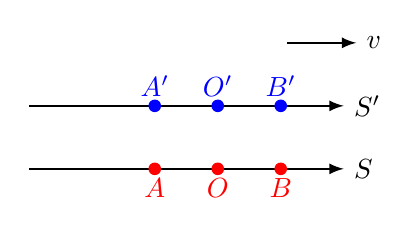
\begin{tikzpicture}[scale=0.8, >=latex]
        \draw [thick, ->] (1,0) -- (6,0) node [right] {$S$};
        \draw [thick, ->] (1,1) -- (6,1) node [right] {$S'$};
        
        \draw [thick, ->] (5.1,2) -- (6.2,2) node [right] {$v$};
        
        \fill [red] (3,0) circle (0.1) node [below] {$A$};
        \fill [red] (4,0) circle (0.1) node [below] {$O$};
        \fill [red] (5,0) circle (0.1) node [below] {$B$};
        
        \fill [blue] (3,1) circle (0.1) node [above] {$A'$};
        \fill [blue] (4,1) circle (0.1) node [above] {$O'$};
        \fill [blue] (5,1) circle (0.1) node [above] {$B'$};
    \end{tikzpicture}
    \caption{「同时」的相对性}
    \label{fig:simultaneity}
\end{figure}

同时,位于 $O(O')$ 处的光源向左右两侧各发射一束光信号。

在 $S$ 系中,$\overline{OA} = \overline{OB} = c t_0$,$A$ 和 $B$ 据此对表。

在 $S'$ 系中,$\overline{O'A} = \overline{O'B} = c t_0$,$A'$ 和 $B'$ 据此对表。

然而在 $S$ 系中的观者认为 $S'$ 系中的对表有问题,因为 $S'$ 系中的光源在向右运动,光信号到达 $A'$ 的时间为
\begin{equation}
    t = \frac{\overline{OA} - v t}{c}
\end{equation}
类似地,光信号到达 $B'$ 的时间为
\begin{equation}
    t = \frac{\overline{OB} + v t}{c}
\end{equation}
即光信号到达 $A'$ 的时间早于到达 $B'$ 的时间,同时是相对的。

\subsubsection{时间间隔的差异)}

在不同参考系中,观察到的光的传播距离不同,而光速不变,因此观察到的时间间隔也不同。

\subsubsection{空间测量的差异}

考虑将一把标准尺放置在 $S'$ 系中,沿 $x'$ 轴方向静止。
在 $S'$ 系中测量该标准尺的长度为 $L_0$。
而在 $S$ 系中测量该标准尺的长度时,需要在\textbf{同一时刻}测量标准尺的两个端点的位置。
因为同时的相对性,空间测量也出现了差异。

\section{狭义相对论时空变换及其推论}

\subsection{狭义相对论时空变换}

考虑两个惯性参考系 $S$ 和 $S'$,其中 $S'$ 以速度 $\bm{v}$ 相对于 $S$ 运动。
在不失一般性的情况下,不妨设 $\bm{v}$ 沿 $x$ 轴正方向。

在开始推导之前,我们要定义一下什么是事件(Event)。
\begin{definition}{事件}{event}
    事件是指在时空中发生的一个特定的现象,可以用一组时空坐标 $(t, x, y, z)$ 来描述。
    即在参考系 $S$ 中,事件发生的时间为 $t$,空间位置为 $(x, y, z)$。
\end{definition}

由于只考虑 $x$ 轴方向的运动,$y$ 和 $z$ 坐标不变,可以认为 $y' = y$,$z' = z$。
设事件在 $S$ 系中的坐标为 $(t, x)$,在 $S'$ 系中的坐标为 $(t', x')$。

首先,$S$ 系中的匀速直线性运动在 $S'$ 系中仍然是匀速直线性运动,即
\begin{equation}
    \bm{a} = 0 \iff \bm{a'} = 0
\end{equation}

因此,时空变换应为线性变换(否则与实验相悖):
\begin{equation}
    \left\{
    \begin{aligned}
        x' &= a_{11} x + a_{12} t \\
        t' &= a_{21} x + a_{22} t
    \end{aligned}
    \right.
    \label{eq:linear-transformation}
\end{equation}

接下来,考虑 $S$ 系与 $S'$ 系地位互换的逆变换 $x' \to -x$,$x \to -x'$,则有
\begin{equation}
    \left\{
    \begin{aligned}
        -x &= a_{11} (-x') + a_{12} t' \\
        t  &= a_{21} (-x') + a_{22} t'
    \end{aligned}
    \right.
    \label{eq:inverse-transformation}
\end{equation}

将 \cref{eq:inverse-transformation} 代入 \cref{eq:linear-transformation},得到
\begin{equation}
    \left\{
    \begin{aligned}
        x' &= a_{11}^2 x' + a_{11} a_{12} t + a_{12} a_{21} x + a_{12} a_{22} t \\
        t' &= -a_{21} a_{11} x' - a_{21} a_{12} t + a_{22} a_{21} x + a_{22}^2 t
    \end{aligned}
    \right.
\end{equation}

比较两式,得到
\begin{equation}
    \left\{
    \begin{aligned}
        a_{11}^2 - a_{12} a_{21} = 1 \\
        a_{11} = a_{22}
    \end{aligned}
    \right.
\end{equation}

再考虑 $S'$ 系中的原点 $O'$ 在 $S$ 系中的运动轨迹,由于 $O'$ 在 $S'$ 系中静止,有
\begin{equation}
    x' = 0 \implies x = -\frac{a_{12}}{a_{11}} t
\end{equation}
因此,$S'$ 系相对于 $S$ 系的速度为
\begin{equation}
    v = -\frac{a_{12}}{a_{11}}
\end{equation}
即
\begin{equation}
    a_{11} v + a_{12} = 0
\end{equation}

最后考虑光速不变原理,在 $S$ 系中,光沿 $x$ 轴正方向传播时,满足 $x = c t$,在 $S'$ 系中应满足 $x' = c t'$。
将 $x = c t$ 和 $x' = c t'$ 代入 \cref{eq:linear-transformation},得到
\begin{equation}
    \left\{
    \begin{aligned}
        c t' &= a_{11} (c t) + a_{12} t \\
        t'   &= a_{21} (c t) + a_{22} t
    \end{aligned}
    \right.
\end{equation}
即
\begin{equation}
    a_{12} = a_{21} c^2
\end{equation}

综上所述,得到
\begin{equation}
    \left\{
    \begin{aligned}
        a_{11}^2 - a_{21}^2 c^2 &= 1 \\
        a_{22} - a_{11} &= 0 \\
        a_{11} v + a_{21} &= 0 \\
        a_{12} - a_{21} c^2 &= 0
    \end{aligned}
    \right.
\end{equation}
解得
\begin{equation}
    \left\{
    \begin{aligned}
        a_{11} &= \frac{1}{\sqrt{1 - \frac{v^2}{c^2}}} \\
        a_{22} &= \frac{1}{\sqrt{1 - \frac{v^2}{c^2}}} \\
        a_{21} &= -\frac{v}{c^2} \frac{1}{\sqrt{1 - \frac{v^2}{c^2}}} \\
        a_{12} &= -v \frac{1}{\sqrt{1 - \frac{v^2}{c^2}}}
    \end{aligned}
    \right.
\end{equation}

因此有如下定理:
\begin{theorem}{狭义相对论时空变换(洛伦兹变换)}{lorentz-transformation}
    设两个惯性参考系 $S$ 和 $S'$,其中 $S'$ 以速度 $\bm{v}$ 相对于 $S$ 运动,且 $\bm{v}$ 沿 $x$ 轴正方向。
    事件在 $S$ 系中的坐标为 $(t, x, y, z)$,在 $S'$ 系中的坐标为 $(t', x', y', z')$,则有如下时空变换关系:
    \begin{equation}
        \left\{
        \begin{aligned}
            x' &= \frac{(x - v t)}{\sqrt{1 - \frac{v^2}{c^2}}} \\
            t' &= \frac{\left(t - \frac{v x}{c^2}\right)}{\sqrt{1 - \frac{v^2}{c^2}}} \\
            y' &= y \\
            z' &= z
        \end{aligned}
        \right.
        \label{eq:lorentz-transformation}
    \end{equation}
\end{theorem}

在这里,我们顺便引入一个重要的概念,即固有时(proper time),即
\begin{definition}{固有时}{proper-time}
    固有时是指在与事件发生的物体共动的参考系中测量到的时间,常用符号 $\tau$ 表示。
    对应的时间间隔 $\Delta \tau$ 被称为固有时间间隔。

    例如,在 $S'$ 系中测量到的时间间隔 $\Delta t'$ 就是事件发生的物体的固有时间间隔,即 $\Delta \tau = \Delta t'$。
\end{definition}


\begin{note}{洛伦兹变换的历史背景}{lorentz-transformation-history}
    洛伦兹变换是洛伦兹(Lorentz)为了解决麦克斯韦方程组的协变性问题(即电磁现象在不同惯性参考系中的形式不变性)而提出的。
    后来由庞加莱(Poincaré)和爱因斯坦(Einstein)进一步发展,成为狭义相对论的核心内容之一。
\end{note}

在实践中,我们经常将上式写成如下形式:
\begin{equation}
    \left\{
    \begin{aligned}
        x' &= \gamma (x - v t) \\
        t' &= \gamma \left(t - \frac{v x}{c^2}\right) \\
        y' &= y \\
        z' &= z
    \end{aligned}
    \right.
\end{equation}
其中,$ \gamma = \frac{1}{\sqrt{1 - \frac{v^2}{c^2}}} $ 称为洛伦兹因子(Lorentz factor)。
而 $ \beta = \frac{v}{c} $ 则是一个无量纲的速度参数,表示物体速度与光速之比。

此外,洛伦兹变换的逆变换为
\begin{equation}
    \left\{
    \begin{aligned}
        x &= \gamma (x' + v t') \\
        t &= \gamma \left(t' + \frac{v x'}{c^2}\right) \\
        y &= y' \\
        z &= z'
    \end{aligned}
    \right.
\end{equation}
推导过程是简单的,即将 $v$ 替换为 $-v$ 即可。

\subsection{狭义相对论时空变换的推论}

\subsubsection{时间膨胀}

考虑 $S'$ 系中的一个时钟静止在 $x' = 0$ 处,测量其两个滴答之间的时间间隔为 $\Delta t' = t_2' - t_1'$。
在 $S$ 系中测量该时钟的时间间隔为 $\Delta t = t_2 - t_1$。

根据洛伦兹变换,有
\begin{equation}
    t' = \gamma \left(t - \frac{v x}{c^2}\right)
\end{equation}
由于时钟在 $S'$ 系中静止在 $x' = 0$处,因此 $x = v t$。
代入上式,得到
\begin{equation}
    t' = \gamma \left(t - \frac{v (v t)}{c^2}\right) = \gamma t \left(1 - \frac{v^2}{c^2}\right) = \frac{t}{\gamma}
\end{equation}
因此,有
\begin{equation}
    \Delta t' = \frac{\Delta t}{\gamma} \implies \Delta t = \gamma \Delta t'
\end{equation}
这表明,在 $S$ 系中测量到的时间间隔 $\Delta t$ 大于在 $S'$ 系中测量到的时间间隔 $\Delta t'$,即时间膨胀效应。

\subsubsection{长度收缩}

考虑 $S'$ 系中的一把标准尺静止在 $x'$ 轴上,测量其长度为 $l_0 = x_2' - x_1'$。
在 $S$ 系中测量该标准尺的长度为 $l = x_2 - x_1$。
根据洛伦兹变换,有
\begin{equation}
    x' = \gamma (x - v t)
\end{equation}

为了在 $S$ 系中测量标准尺的长度,需要在同一时刻测量其两个端点的位置,即 $t_1 = t_2$。
因此,有
\begin{equation}
    x_1' = \gamma (x_1 - v t_1)
\end{equation}
\begin{equation}
    x_2' = \gamma (x_2 - v t_2)
\end{equation}
两式相减,得到
\begin{equation}
    l_0 = x_2' - x_1' = \gamma (x_2 - x_1) = \gamma l
\end{equation}
因此,有
\begin{equation}
    l = \frac{l_0}{\gamma}
\end{equation}
这表明,在 $S$ 系中测量到的长度 $l$ 小于在 $S'$ 系中测量到的长度 $l_0$,即长度收缩效应。

\subsubsection{因果律与时序关系的保持}

考虑两个事件 $A$ 和 $B$,在 $S$ 系中的时空坐标分别为 $(t_A, x_A)$ 和 $(t_B, x_B)$。
定义事件 $A$ 发生在事件 $B$ 之前,即 $t_A < t_B$。
根据洛伦兹变换,有
\begin{equation}
    t' = \gamma \left(t - \frac{v x}{c^2}\right)
\end{equation}
因此,有
\begin{equation}
    t_A' = \gamma \left(t_A - \frac{v x_A}{c^2}\right)
\end{equation}
\begin{equation}
    t_B' = \gamma \left(t_B - \frac{v x_B}{c^2}\right)
\end{equation}
两式相减,得到
\begin{equation}
    t_B' - t_A' = \gamma \left((t_B - t_A) - \frac{v (x_B - x_A)}{c^2}\right)
\end{equation}

为了保证因果律不被破坏,即事件 $A$ 发生在事件 $B$ 之前在所有惯性参考系中都成立,需要满足
\begin{equation}
    (t_B - t_A) - \frac{v (x_B - x_A)}{c^2} > 0
\end{equation}
即
\begin{equation}
    t_B - t_A > \frac{v (x_B - x_A)}{c^2}
\end{equation}
这表明,只要事件 $A$ 和事件 $B$ 之间的时空间隔是类时的(即 $c^2 (t_B - t_A)^2 > (x_B - x_A)^2$),则因果律在所有惯性参考系中都得到保持。
只要观者所在的惯性参考系的速度 $v$ 小于光速 $c$,事件的时序关系不会被改变。

\subsubsection{速度变换公式}

考虑质点相对 $S$,$S'$ 系的速度分别为
\begin{equation}
    \bm{u} : u_x = \frac{d x}{d t} , \quad u_y = \frac{d y}{d t} , \quad u_z = \frac{d z}{d t}
\end{equation}
\begin{equation}
    \bm{u'} : u_x' = \frac{d x'}{d t'} , \quad u_y' = \frac{d y'}{d t'} , \quad u_z' = \frac{d z'}{d t'}
\end{equation}

根据洛伦兹变换,有
\begin{equation}
    x' = \gamma (x - v t)
\end{equation}
\begin{equation}
    t' = \gamma \left(t - \frac{v x}{c^2}\right)
\end{equation}
对两式分别微分,得到
\begin{equation}
    \d x' = \gamma (\d x - v \d t)
\end{equation}
\begin{equation}
    \d t' = \gamma \left(\d t - \frac{v \d x}{c^2}\right)
\end{equation}
因此,有
\begin{equation}
    u_x' = \frac{ \d x'}{\d t'} = \frac{\gamma (\d x - v \d t)}{\gamma \left(\d t - \frac{v \d x}{c^2}\right)} = \frac{\d x - v \d t}{\d t - \frac{v \d x}{c^2}}
\end{equation}
将 $\d x = u_x \d t$ 代入上式,得到
\begin{equation}
    u_x' = \frac{u_x - v}{1 - \frac{v u_x}{c^2}}
\end{equation}
类似地,有
\begin{equation}
    u_y' = \frac{\d y'}{\d t'} = \frac{\d y}{\gamma \left(\d t - \frac{v \d x}{c^2}\right)} = \frac{u_y \d t}{\gamma \left(\d t - \frac{v u_x \d t}{c^2}\right)} = \frac{u_y}{\gamma \left(1 - \frac{v u_x}{c^2}\right)}
\end{equation}
\begin{equation}
    u_z' = \frac{\d z'}{\d t'} = \frac{\d z}{\gamma \left(\d t - \frac{v \d x}{c^2}\right)} = \frac{u_z \d t}{\gamma \left(\d t - \frac{v u_x \d t}{c^2}\right)} = \frac{u_z}{\gamma \left(1 - \frac{v u_x}{c^2}\right)}
\end{equation}

综上所述,有如下定理:
\begin{theorem}{狭义相对论速度变换公式}{velocity-transformation}
    设质点相对 $S$,$S'$ 系的速度分别为 $\bm{u}$ 和 $\bm{u'}$,则有如下速度变换关系:
    \begin{equation}
        \left\{
        \begin{aligned}
            u_x' &= \frac{u_x - v}{1 - \frac{v u_x}{c^2}} \\
            u_y' &= \frac{u_y}{\gamma \left(1 - \frac{v u_x}{c^2}\right)} \\
            u_z' &= \frac{u_z}{\gamma \left(1 - \frac{v u_x}{c^2}\right)}
        \end{aligned}
        \right.
    \end{equation}
    其中,$\gamma = \frac{1}{\sqrt{1 - \frac{v^2}{c^2}}}$。
\end{theorem}

类似地,速度变换的逆变换为
\begin{equation}
    \left\{
    \begin{aligned}
        u_x &= \frac{u_x' + v}{1 + \frac{v u_x'}{c^2}} \\
        u_y &= \frac{u_y'}{\gamma \left(1 + \frac{v u_x'}{c^2}\right)} \\
        u_z &= \frac{u_z'}{\gamma \left(1 + \frac{v u_x'}{c^2}\right)}
    \end{aligned}
    \right.
\end{equation}

\begin{note}{速度变换公式的意义}{velocity-transformation-meaning}
    速度变换公式表明,在狭义相对论中,速度的叠加不再是简单的代数和,而是受到光速不变原理的限制。
    这确保了无论在任何惯性参考系中,物体的速度都不会超过光速 $c$。
\end{note}

\begin{note}{速度变换公式与双曲函数的关系}{velocity-transformation-hyperbolic}
    在这里,你可能会发现这个速度变换公式与 $\tan x$ 的加法公式非常相似,这并非巧合。
    实际上,狭义相对论中的速度变换可以类比为双曲正切函数的加法公式,这揭示了狭义相对论中速度空间的几何结构。

    具体来说,设 $u = c \cdot \tanh \phi$ 和 $v = c \cdot \tanh \psi$,则速度变换公式可以写成
    \begin{equation}
        \tanh(\phi + \psi) = \frac{\tanh \phi + \tanh \psi}{1 + \tanh \phi \tanh \psi}
    \end{equation}

    这表明,狭义相对论中的速度变换实际上对应于双曲角的加法,这进一步强调了狭义相对论中时空的双曲几何性质。
    而此处的 $\phi$ 和 $\psi$ 被称为快度角(boost angle)或快度参数(rapidity)。
\end{note}





下面给出一个例子,即加速度变换公式的推导。
\begin{example}{加速度变换公式的推导}{acceleration-transformation-derivation}
    设质点相对 $S$,$S'$ 系的加速度分别为
    \begin{equation}
        \bm{a} : a_x = \frac{d u_x}{d t} , \quad a_y = \frac{d u_y}{d t} , \quad a_z = \frac{d u_z}{d t}
    \end{equation}
    \begin{equation}
        \bm{a'} : a_x' = \frac{d u_x'}{d t'} , \quad a_y' = \frac{d u_y'}{d t'} , \quad a_z' = \frac{d u_z'}{d t'}
    \end{equation}

    \textbf{解}:

    根据速度变换公式,有
    \begin{equation}
        u_x' = \frac{u_x - v}{1 - \frac{v u_x}{c^2}}
    \end{equation}
    对上式分别对 $t$ 和 $t'$ 微分,得到
    \begin{equation}
        \d u_x' = \frac{(1 - \frac{v^2}{c^2}) \d u_x}{\left(1 - \frac{v u_x}{c^2}\right)^2}
    \end{equation}
    \begin{equation}
        \d t' = \frac{(1 - \frac{v u_x}{c^2}) \d t}{\sqrt{1 - \frac{v^2}{c^2}}}
    \end{equation}
    因此,有
    \begin{equation}
        a_x' = \frac{\d u_x'}{\d t'} = \frac{\frac{(1 - \frac{v^2}{c^2}) \d u_x}{\left(1 - \frac{v u_x}{c^2}\right)^2}}{\frac{(1 - \frac{v u_x}{c^2}) \d t}{\sqrt{1 - \frac{v^2}{c^2}}}} = \frac{(1 - \frac{v^2}{c^2})^{3/2} a_x}{\left(1 - \frac{v u_x}{c^2}\right)^3}
    \end{equation}
    类似地,有
    \begin{equation}
        \d u_y' = \frac{\partial u_y'}{\partial u_y} \d u_y + \frac{\partial u_y'}{\partial u_x} \d u_x = \frac{\d u_y}{\gamma \left(1 - \frac{v u_x}{c^2}\right)} + \frac{v u_y \d u_x}{c^2 \gamma \left(1 - \frac{v u_x}{c^2}\right)^2}
    \end{equation}
    因此,有
    \begin{equation}
        a_y' = \frac{\d u_y'}{\d t'} = \frac{\frac{\d u_y}{\gamma \left(1 - \frac{v u_x}{c^2}\right)} + \frac{v u_y \d u_x}{c^2 \gamma \left(1 - \frac{v u_x}{c^2}\right)^2}}{\frac{(1 - \frac{v u_x}{c^2}) \d t}{\sqrt{1 - \frac{v^2}{c^2}}}} = \frac{a_y}{\gamma^2 \left(1 - \frac{v u_x}{c^2}\right)^2} + \frac{v u_y a_x}{c^2 \gamma^2 \left(1 - \frac{v u_x}{c^2}\right)^3}
    \end{equation}
    同理,有
    \begin{equation}
        a_z' = \frac{a_z}{\gamma^2 \left(1 - \frac{v u_x}{c^2}\right)^2} + \frac{v u_z a_x}{c^2 \gamma^2 \left(1 - \frac{v u_x}{c^2}\right)^3}
    \end{equation}

    逆变换类似,有
    \begin{equation}
        a_x = \frac{(1 - \frac{v^2}{c^2})^{3/2} a_x'}{\left(1 + \frac{v u_x'}{c^2}\right)^3}
    \end{equation}
    \begin{equation}
        a_y = \frac{a_y'}{\gamma^2 \left(1 + \frac{v u_x'}{c^2}\right)^2} - \frac{v u_y' a_x'}{c^2 \gamma^2 \left(1 + \frac{v u_x'}{c^2}\right)^3}
    \end{equation}
    \begin{equation}
        a_z = \frac{a_z'}{\gamma^2 \left(1 + \frac{v u_x'}{c^2}\right)^2} - \frac{v u_z' a_x'}{c^2 \gamma^2 \left(1 + \frac{v u_x'}{c^2}\right)^3}
    \end{equation}
    $\hfill \blacksquare $

    在相对论中,加速度的变换关系比经典力学中的更为复杂,反映了狭义相对论对时间和空间测量的影响。
    仅当 $\bm{a}' = 0$ 时,才有 $\bm{a} = 0$,即匀速直线运动在所有惯性参考系中保持不变。
    此外,它还有三个特征:
    \begin{itemize}
        \item 一般情况下,$\bm{a} \neq \bm{a}'$;
        \item 加速度分量之间存在耦合;
        \item 质点加速度的变换与质点速度有关。
    \end{itemize}
\end{example}

\section{狭义相对论动力学}

\subsection{引入}

牛顿力学中物体的质量 $m$ 和物体所受力 $\bm{F}$ 一起由关系式 $ \bm{F} = m \bm{a} $ 定义,大量实验对定义的认可使得关系式 $ \bm{F} = m \bm{a}$ 成为定律。
定律中的 $m$ 不随物体的运动状态发生变化,是一个参考系不变量。
经典理论中 $\bm{a}$ 是惯性系不变量,于是牛顿定律的惯性系不变性要求 $\bm{F}$ 也是惯性系不变量。
经典力学涉及的诸多真实力如牛顿万有引力、重力、浮力、摩擦力、弹性力等在当时的实验精度范围内已被证实都是惯性系不变量。

爱因斯坦获义相对论时空度量关系的建立,揭示出除非加速度为零,否则 $a$ 不是惯性系不变量。
面对这一结论,显然不能不加论证地判定在狭义相对论中 $m$、$\bm{F}$ 仍然可以是惯性系不变量,而是需要一般地考察 $m$、$\bm{F}$ 的惯性系变换关系。
另一方面,在狭义相对论中也不能不加论证地认可,以 $ \bm{F} = m \bm{a} $ 形式表述的牛顿第二定律仍然满足相对性原理的要求。
总之,在狭义相对论的动力学内容中,一是要找出 $m$、$\bm{F}$ 的惯性系变换式,二是要建立符合相对性原理要求的牛顿第二定律。

完成上述工作的途径不是唯一的。例如可在改造牛顿第二定律之前,先设定与外界无相
互作用的物质系统其总能量(包括机械能、热能\ldots)和动量分别守恒或者改为设定这样的系统其总质量和动量分别守恒。
而后,通过两个全同质点的弹性碰撞或完全非弹性碰撞,简捷地得到质点质量 $m$ 随其运动速度 $v$ 的变化关系,实质上也就是得到了质量的惯性系变换式。
牛顿第二定律表达式 $ \bm{F} = m \bm{a} $ 中 $m$ 的不变性既然已被否定,便改取表达式 $\bm{F} = \frac{\d \bm{p}}{\d t}$ 来考察它的惯性系不变性和 $\bm{F}$ 的惯性系变换式。

狭义相对论的创建源于电作用理论。
如前所述,爱因斯坦第一篇相对论论文的标题定为《论动体的电动力学》,全篇宗旨就是以新建的狭义相对论时空变换为基础,
从理论上证明麦克斯韦场方程满足相对性原理要求即具有惯性系不变性,同时导得了电磁场量的惯性系变换式。

经过综合考量,笔者便在此处忠实的记录下这两种推导方法。

\subsection{从力学的角度推导\texorpdfstring{\cite{zhaokaihua2004}}{}}

\subsubsection{动量、质量与速度的关系}

首先,我们仍然定义一个质点的动量 $\bm{p}$ 是一个与它的速度 $\bm{v}$ 成正比的矢量,即
\begin{equation}
    \bm{p} = m \bm{v}
\end{equation}
其中,式中的比例系数仍定义为质点的质量 $m$。

不过由于在数量上,质点的动量 $\bm{p}$ 不再与速度 $\bm{v}$ 成简单的正比关系,而是与速度 $\bm{v}$ 的大小有关。
因此,质点的质量 $m$ 也不再是一个常量,而是与质点的速度 $\bm{v}$ 的大小有关。
又由于空间的各向同性,我们认为质点的质量 $m$ 只能与速度 $\bm{v}$ 的大小 $v$ 有关,即 $m = m(v)$。
接下来,我们要确定质点质量 $m$ 随速度 $v$ 的变化关系。

我们考虑一个例子——全同粒子的完全非弹性碰撞。
考虑 $A$、$B$ 两个全同粒子正碰之后成为一个复合粒子。
我们从两个参考系 $S$ 和 $S'$ 来分析这个碰撞过程。
在 $S$ 系中,粒子 $B$ 静止不动,粒子 $A$ 以速度 $v$ 向右运动。
它们的质量分别为 $m_B = m_0$ 和 $m_A = m(v)$。
碰撞之后,复合粒子以速度 $u$ 向右运动。

在 $S'$ 系中,粒子 $A$ 静止不动,粒子 $B$ 以速度 $-v'$ 向左运动。
它们的质量分别为 $m_A = m_0$ 和 $m_B = m(v)$。
碰撞之后,复合粒子以速度 $u'$ 向右运动。

显然,$S$ 系相对于 $S'$ 系的速度为 $v$。
设碰撞之后复合粒子的质量为 $M$,在 $S$ 系中的速度为 $u$,在 $S'$ 系中的速度为 $u'$,依对称性可以看出 $u = -u'$。

根据动量守恒定律,我们有
\begin{equation}
    m(v) v = M(u) u
\end{equation}
根据质量(实际上是能量)守恒定律,我们有
\begin{equation}
    m(v) + m_0 = M(u)
\end{equation}

由此得
\begin{equation}
    \frac{M(u)}{m(v)} = \frac{m(v) + m_0}{m(v)} = \frac{v}{u}
\end{equation}

另一方面,根据相对论速度变换公式,我们有
\begin{equation}
    u' = -u = \frac{u - v}{1 - \frac{v u}{c^2}} \implies \left(\frac{v}{u}\right)^2 - 2 \cdot \frac{v}{u} + \frac{v^2}{c^2} = 0
\end{equation}
解得
\begin{equation}
    \frac{v}{u} = 1 \pm \sqrt{1 - \frac{v^2}{c^2}}
\end{equation}

因为 $\frac{v}{u} > 1$,所以取正号,有
\begin{equation}
    \frac{M(u)}{m(v)} = \frac{m(v) + m_0}{m(v)} = 1 + \sqrt{1 - \frac{v^2}{c^2}}
\end{equation}
解得
\begin{equation}
    m(v) = \frac{m_0}{\sqrt{1 - \frac{v^2}{c^2}}}
\end{equation}

因此,有如下定理:
\begin{theorem}{狭义相对论质量公式}{relativistic-mass}
    设质点的静止质量为 $m_0$,则当质点以速度 $v$ 运动时,其质量 $m$ 为
    \begin{equation}
        m = \frac{m_0}{\sqrt{1 - \frac{v^2}{c^2}}}
    \end{equation}
\end{theorem}
在此之后,我们称式中的 $m$ 为质点的相对论质量或动质量,而 $m_0$ 则称为质点的静止质量或固有质量。

相应的,质点的动量 $\bm{p}$ 为
\begin{equation}
    \bm{p} = \frac{m_0 \bm{v}}{\sqrt{1 - \frac{v^2}{c^2}}} = \gamma m_0 \bm{v}
\end{equation}

\subsubsection{力、功与动能}

再考虑动能的表达式
\begin{equation}
    \begin{aligned}
        E_k = \int_{0}^{l} \bm{F} \cdot \d \bm{s} = \int_{0}^{v} \bm{F} \cdot \frac{\d \bm{s}}{\d t} \d t \\
        = \int_{0}^{v} \frac{\d \bm{p}}{\d t} \cdot \bm{v} \d t = \int_{0}^{v} \bm{v} \cdot \d \bm{p} \\
        = \int_{0}^{v} v \d \left(\frac{m_0 v}{\sqrt{1 - \frac{v^2}{c^2}}}\right) \\
        = \left. \frac{m_0 \bm{v} \cdot \bm{v}}{\sqrt{1 - \frac{v^2}{c^2}}} \right|_{0}^{v} -
        m_0 \int_{0}^{v} \frac{\bm{v} \cdot \d \bm{v}}{\sqrt{1 - \frac{v^2}{c^2}}} \\
        = \frac{m_0 v^2}{\sqrt{1 - \frac{v^2}{c^2}}} + m_0 c^2 \left(\sqrt{1 - \frac{v^2}{c^2}} - 1\right) \\
        = m_0 c^2 \left(\frac{1}{\sqrt{1 - \frac{v^2}{c^2}}} - 1\right)
    \end{aligned}
\end{equation}

因此,有如下定理:
\begin{theorem}{狭义相对论动能公式}{relativistic-kinetic-energy}
    设质点的静止质量为 $m_0$,当质点以速度 $v$ 运动时,其动能 $E_k$ 为
    \begin{equation}
        E_k = (\gamma - 1) m_0 c^2
    \end{equation}
    其中,$\gamma = \frac{1}{\sqrt{1 - \frac{v^2}{c^2}}}$。
\end{theorem}

在 $v^2 / c^2 \ll 1$ 的情况下,将上式展开,有
\begin{equation}
    E_k = \frac{1}{2} m_0 v^2 + \frac{3}{8} m_0 \frac{v^4}{c^2} + \cdots
\end{equation}
显然,在低速极限下,狭义相对论动能公式退化为经典力学动能公式 $E_k = \frac{1}{2} m_0 v^2$。

\subsubsection{质能关系}

在此基础上,我们可以定义质点的总能量 $E$ 为
\begin{equation}
    E = E_k + m_0 c^2 = \gamma m_0 c^2
\end{equation}

\begin{theorem}{狭义相对论能量公式}{relativistic-energy}
    设质点的静止质量为 $m_0$,当质点以速度 $v$ 运动时,其总能量 $E$ 为
    \begin{equation}
        E = \gamma m_0 c^2
    \end{equation}
    其中,$\gamma = \frac{1}{\sqrt{1 - \frac{v^2}{c^2}}}$。
\end{theorem}

\begin{note}{质能关系}{mass-energy-equivalence}
    质点的总能量 $E$ 和质量 $m$ 之间存在如下关系:
    \begin{equation}
        E = m c^2
    \end{equation}
    这表明质量和能量是等价的,可以相互转换。
    这一结论在核反应和粒子物理中得到了广泛的验证。
\end{note}

\subsubsection{能量与动量的关系}

最后我们介绍一下动质能关系
\begin{theorem}{狭义相对论动质能关系}{relativistic-energy-momentum-relation}
    设质点的静止质量为 $m_0$,当质点以速度 $v$ 运动时,其总能量 $E$ 和动量 $\bm{p}$ 满足如下关系:
    \begin{equation}
        E^2 = p^2 c^2 + m_0^2 c^4
    \end{equation}
\end{theorem}

\subsection{从电动力学的角度推导\texorpdfstring{\cite{shuyousheng2005}}{}}

\subsubsection{力的定义与变换}

麦克斯韦场方程是以 $\bm{E}$ 和 $\bm{B}$ 已有度量定义为前提的,逻辑上可以将带电质点在电作用场中的受力公式
\begin{equation}
    \bm{F} = q (\bm{E} + \bm{u} \times \bm{B})
    \label{eq:relativistic-force-definition}
\end{equation}
处理为对 $\bm{E}$ 和 $\bm{B}$ 的定义式,式中 $q$ 是带电质点的电量,$\bm{u}$ 是带电质点的运动速度。
\cref{eq:relativistic-force-definition} 的含义是将电作用场分解成电场和磁场两部分。
其中电场给电荷 $q$ 的作用力 $\bm{F}_e$ 与带电质点运动状态无关,力的结构式 $\bm{F}_e = q \bm{E}$ 中的 $\bm{E}$ 即为电场参与力构造的因素量。
磁场仅对运动电荷施以附加的作用力 $\bm{F}_m$,力的结构式 $\bm{F}_m = q \bm{u} \times \bm{B}$ 中的 $\bm{B}$ 即为磁场参与力构造的因素量。
经典理论中,$\bm{F}$ 已在质点动力学中给出度量定义。

狭义相对论中,在尚未完成对牛顿三定律的检查和修正工作时逻辑上也可以在电作用理论框架内,将 \cref{eq:relativistic-force-definition} 处理成同时给出$\bm{F}$、$q$、$\bm{E}$、$\bm{B}$度量定义的基本公式。
电作用理论中认定 $q$ 是运动不变量这也是可以理解的。
宏观物体均由原子构成原子中电子的电量若因电子绕核高速运动而发生变化原子便不再是电中性的原子间会相互排斥,宏观物体很难稳定,这与事实不符。

\cref{eq:relativistic-force-definition} 是惯性系不变式,符号右边的 $q$ 是惯性系不变量,速度 $\bm{u}$ 的惯性系变换式已经给出,
那么在获得 $\bm{E}$ 和 $\bm{B}$ 的惯性系变换式后,便可导得力 $\bm{F}$ 的变换式。

我们首先推导 $\bm{E}$ 和 $\bm{B}$ 的惯性系变换式。

先考虑麦克斯韦方程组中的
\begin{equation}
    \nabla \cdot \bm{B} = 0 , \quad \nabla \times \bm{E} = - \frac{\partial \bm{B}}{\partial t}
\end{equation}
即
\begin{equation}
    \left\{
    \begin{aligned}
        & \frac{\partial B_x}{\partial x} + \frac{\partial B_y}{\partial y} + \frac{\partial B_z}{\partial z} = 0 \\
        & \frac{\partial E_z}{\partial y} - \frac{\partial E_y}{\partial z} = - \frac{\partial B_x}{\partial t} \\
        & \frac{\partial E_x}{\partial z} - \frac{\partial E_z}{\partial x} = - \frac{\partial B_y}{\partial t} \\
        & \frac{\partial E_y}{\partial x} - \frac{\partial E_x}{\partial y} = - \frac{\partial B_z}{\partial t}
    \end{aligned}
    \right.
    \label{eq:maxwell-equations-1}
\end{equation}

由 \cref{eq:lorentz-transformation} 可得
\begin{equation}
    \left\{
    \begin{aligned}
        & \frac{\partial }{\partial x} = \gamma \left(\frac{\partial }{\partial x'} - \frac{v}{c^2} \frac{\partial }{\partial t'}\right) \\
        & \frac{\partial }{\partial y} = \frac{\partial }{\partial y'} \\
        & \frac{\partial }{\partial z} = \frac{\partial }{\partial z'} \\
        & \frac{\partial }{\partial t} = \gamma \left(\frac{\partial }{\partial t'} - v \frac{\partial }{\partial x'}\right)
    \end{aligned}
    \right.
\end{equation}

代入 \cref{eq:maxwell-equations-1},可得
\begin{equation}
    \left\{
    \begin{aligned}
        & \frac{1}{\sqrt{1 - \frac{v^2}{c^2}}} \frac{\partial B_x}{\partial x'} - \frac{v}{c^2 \sqrt{1 - \frac{v^2}{c^2}}} \frac{\partial B_x}{\partial t'} + \frac{\partial B_y}{\partial y'} + \frac{\partial B_z}{\partial z'} = 0 \\
        & \frac{\partial E_z}{\partial y'} - \frac{\partial E_y}{\partial z'} = - \frac{1}{\sqrt{1 - \frac{v^2}{c^2}}} \frac{\partial B_x}{\partial t'} + \frac{v}{\sqrt{1 - \frac{v^2}{c^2}}} \frac{\partial B_x}{\partial x'} \\
        & \frac{1}{\sqrt{1 - \frac{v^2}{c^2}}} \frac{\partial E_x}{\partial z'} - \frac{\partial E_z}{\partial x'} = - \frac{1}{\sqrt{1 - \frac{v^2}{c^2}}} \frac{\partial B_y}{\partial t'} + \frac{v}{\sqrt{1 - \frac{v^2}{c^2}}} \frac{\partial B_y}{\partial x'} \\
        & \frac{\partial E_y}{\partial x'} - \frac{1}{\sqrt{1 - \frac{v^2}{c^2}}} \frac{\partial E_x}{\partial y'} + \frac{v}{c^2 \sqrt{1 - \frac{v^2}{c^2}}} \frac{\partial E_x}{\partial t'} = - \frac{1}{\sqrt{1 - \frac{v^2}{c^2}}} \frac{\partial B_z}{\partial t'} + \frac{v}{\sqrt{1 - \frac{v^2}{c^2}}} \frac{\partial B_z}{\partial x'}
    \end{aligned}
    \right.
\end{equation}
从前两个公式中,先消去含 $\frac{\partial}{\partial t'}$ 的项,再消去含 $\frac{\partial}{\partial x'}$ 的项,可以得出两个等价的表达式。
对后两个公式,合并同类项,也可以得出两个等价的表达式。由此得出
\begin{equation}
    \left\{
    \begin{aligned}
        & \frac{\partial B_x}{\partial x'} + \frac{\partial}{\partial y'} \left[ \frac{1}{\sqrt{1 - \frac{v^2}{c^2}}} (B_y + \frac{v}{c^2} E_z) \right] + \frac{\partial}{\partial z'} \left[ \frac{1}{\sqrt{1 - \frac{v^2}{c^2}}} (B_z - \frac{v}{c^2} E_y) \right] = 0 \\
        & \frac{\partial}{\partial y'} \left[ \frac{1}{\sqrt{1 - \frac{v^2}{c^2}}} (E_z + v B_y) \right] - \frac{\partial}{\partial z'} \left[ \frac{1}{\sqrt{1 - \frac{v^2}{c^2}}} (E_y - v B_z) \right] = - \frac{\partial B_x}{\partial t'} \\
        & - \frac{\partial}{\partial x'} \left[ \frac{1}{\sqrt{1 - \frac{v^2}{c^2}}} (E_z + v B_y) \right] + \frac{\partial E_x}{\partial z'} = - \frac{\partial}{\partial t'} \left[ \frac{1}{\sqrt{1 - \frac{v^2}{c^2}}} (B_y + \frac{v}{c^2} E_z) \right] \\
        & \frac{\partial}{\partial x'} \left[ \frac{1}{\sqrt{1 - \frac{v^2}{c^2}}} (E_y - v B_z) \right] - \frac{\partial E_x}{\partial y'} = - \frac{\partial}{\partial t'} \left[ \frac{1}{\sqrt{1 - \frac{v^2}{c^2}}} (B_z - \frac{v}{c^2} E_y) \right]
        \end{aligned}
    \right.
\end{equation}

比较上式与 \cref{eq:maxwell-equations-1} 在 $S'$ 系中的形式,可得
\begin{equation}
    \left\{
    \begin{aligned}
        & B_x' = B_x \\
        & B_y' = \frac{1}{\sqrt{1 - \frac{v^2}{c^2}}} (B_y + \frac{v}{c^2} E_z) \\
        & B_z' = \frac{1}{\sqrt{1 - \frac{v^2}{c^2}}} (B_z - \frac{v}{c^2} E_y) \\
        & E_x' = E_x \\
        & E_y' = \frac{1}{\sqrt{1 - \frac{v^2}{c^2}}} (E_y - v B_z) \\
        & E_z' = \frac{1}{\sqrt{1 - \frac{v^2}{c^2}}} (E_z + v B_y)
    \end{aligned}
    \right.
\end{equation}

\medskip

为了导出力 $\bm{F}$ 的惯性系变换式,先用 $\bm{u}$ 点乘 \cref{eq:relativistic-force-definition},得
\begin{equation}
    \bm{F} \cdot \bm{u} = q \bm{E} \cdot \bm{u} + q (\bm{u} \times \bm{B}) \cdot \bm{u} = q \bm{E} \cdot \bm{u}
\end{equation}
同理,在 $S'$ 系中,有
\begin{equation}
    \bm{F'} \cdot \bm{u'} = q \bm{E'} \cdot \bm{u'}
\end{equation}

考虑 $x'$ 方向的力分量 $F_x$:
\begin{equation}
    F_x' = q \left( E_x' + u_y' B_z' - u_z' B_y' \right)
\end{equation}
代入 $\bm{E'}$、$\bm{B'}$ 和 $\bm{u'}$ 的惯性系变换式,得
\begin{equation}
    \begin{aligned}
        F_x' & = q \left[ E_x + \frac{u_y \left( B_z - \frac{v}{c^2} E_y \right)}{1 - \frac{v}{c^2} u_x} - \frac{u_z \left( B_y + \frac{v}{c^2} E_z \right)}{1 - \frac{v}{c^2} u_x} \right] \\
        & = \frac{q}{1 - \frac{v}{c^2} u_x} \left( E_x + u_y B_z - u_z B_y - \frac{v}{c^2} (u_x E_x + u_y E_y + u_z E_z) \right) \\
        & = \frac{1}{1 - \frac{v}{c^2} u_x} \left( F_x - \frac{v}{c^2} q \bm{u} \cdot \bm{E} \right)
    \end{aligned}
\end{equation}
即
\begin{equation}
    F_x' = \frac{F_x - \frac{v}{c^2} \bm{F} \cdot \bm{u}}{1 - \frac{v}{c^2} u_x}
\end{equation}

类似地,有
\begin{equation}
    F_y' = \frac{\sqrt{1 - \frac{v^2}{c^2}} F_y}{1 - \frac{v}{c^2} u_x}
\end{equation}
\begin{equation}
    F_z' = \frac{\sqrt{1 - \frac{v^2}{c^2}} F_z}{1 - \frac{v}{c^2} u_x}
\end{equation}

综上所述,力 $\bm{F}$ 的惯性系变换式为
\begin{equation}
    \left\{
    \begin{aligned}
        & F_x' = \frac{F_x - \frac{v}{c^2} \bm{F} \cdot \bm{u}}{1 - \frac{v}{c^2} u_x} \\
        & F_y' = \frac{\sqrt{1 - \frac{v^2}{c^2}} F_y}{1 - \frac{v}{c^2} u_x} \\
        & F_z' = \frac{\sqrt{1 - \frac{v^2}{c^2}} F_z}{1 - \frac{v}{c^2} u_x}
    \end{aligned}
    \right.
    \label{eq:relativistic-force-transformation}
\end{equation}

逆变换为
\begin{equation}
    \left\{
    \begin{aligned}
        & F_x = \frac{F_x' + \frac{v}{c^2} \bm{F'} \cdot \bm{u'}}{1 + \frac{v}{c^2} u_x'} \\
        & F_y = \frac{\sqrt{1 - \frac{v^2}{c^2}} F_y'}{1 + \frac{v}{c^2} u_x'} \\
        & F_z = \frac{\sqrt{1 - \frac{v^2}{c^2}} F_z'}{1 + \frac{v}{c^2} u_x'}
    \end{aligned}
    \right.
\end{equation}

\subsubsection{牛顿三定律的修正}

\begin{itemize}
    \item 牛顿第一定律
    牛顿第一定律在狭义相对论中仍然成立,即在没有外力作用下,质点保持匀速直线运动状态。
    \item 牛顿第二定律
    狭义相对论中,改取牛顿第二定律的原始形式,即
    \begin{equation}
        \bm{F} = \frac{\d \bm{p}}{\d t}
        \label{eq:relativistic-newton-second-law}
    \end{equation}
    其中,$\bm{p}$ 是质点的动量。
    $\d t'$ 和 $\bm{F}$ 的惯性系变换式已经给出,对于给定的 $S$ 系中的质点动量 $\bm{P}$,如果能够找到对应的 $S'$ 系中的质点动量 $\bm{p'}$,使得
    \begin{equation}
        \bm{F'} = \frac{\d \bm{p'}}{\d t'}
    \end{equation}
    成立,那么在 \cref{eq:relativistic-newton-second-law} 表述形式上便是惯性系不变的。
    当然,这样修正的牛顿第二定律是否正确,还需经过实验验证。
    \item 牛顿第三定律
    狭义相对论中,如果牛顿第三定律仍然成立,便要求在 $S$ 系中的一对力若是 $\bm{F_1} + \bm{F_2} = \bm{0}$,
    那么变换到 $S'$ 系也必有 $\bm{F_1} + \bm{F_2} = \bm{0}$,据力的变换式 \cref{eq:relativistic-force-transformation}很易举出反例。

    狭义相对论中牛顿第三定律虽然不能成立,但在狭义相对论之前已经建立的普遍的动量守恒定律(即任何一个与外界无相互作用的系统其动量守恒)仍然成立。
\end{itemize}

\subsubsection{动量及能量变换}

根据牛顿第二定律的修正形式 \cref{eq:relativistic-newton-second-law},可得质点动量定理
\begin{equation}
    \bm{F} \d t = \d \bm{p}
    \label{eq:relativistic-momentum-theorem}
\end{equation}

同时补充定义,假设力 $\bm{F}$ 对质点所做的功仍然等于质点能量的增量,即
\begin{equation}
    \bm{F} \cdot \d \bm{l} = \d E
    \label{eq:relativistic-work-energy-theorem}
\end{equation}

假设 \cref{eq:relativistic-momentum-theorem} 和 \cref{eq:relativistic-work-energy-theorem} 都是惯性系不变的,则有
\begin{equation}
    \d p_x' = F_x' \d t' = \frac{F_x - \frac{v}{c^2} \bm{F} \cdot \bm{u}}{1 - \frac{v}{c^2} u_x} \cdot \frac{\d t - \frac{v}{c^2} \d x}{\sqrt{1 - \frac{v^2}{c^2}}}
\end{equation}
将 $\d x = u_x \d t$ 和 $\bm{u} \d t = \d \bm{l}$ 代入上式,得
\begin{equation}
    \d p_x' = \frac{1}{\sqrt{1 - \frac{v^2}{c^2}}} \left( \d p_x - \frac{v}{c^2} \d E \right)
\end{equation}
积分后得
\begin{equation}
    p_x' = \frac{p_x - \frac{v}{c^2} E}{\sqrt{1 - \frac{v^2}{c^2}}} + C_1
\end{equation}
其中 $C_1$ 是积分常数,可以令 $C_1 = 0$,再在实验中验证这个选择的正确性。

同样地,有
\begin{equation}
    \d y' = F_y' \d t' = \frac{\sqrt{1 - \frac{v^2}{c^2}} F_y}{1 - \frac{v}{c^2} u_x} \cdot \frac{\d t - \frac{v}{c^2} \d x}{\sqrt{1 - \frac{v^2}{c^2}}} = F_y \d t = \d p_y
\end{equation}
\begin{equation}
    \d z' = F_z' \d t' = \frac{\sqrt{1 - \frac{v^2}{c^2}} F_z}{1 - \frac{v}{c^2} u_x} \cdot \frac{\d t - \frac{v}{c^2} \d x}{\sqrt{1 - \frac{v^2}{c^2}}} = F_z \d t = \d p_z
\end{equation}

积分后,令积分常数为零,得
\begin{equation}
    p_y' = p_y
\end{equation}
\begin{equation}
    p_z' = p_z
\end{equation}

同样地,对于能量的变换,有
\begin{equation}
    \d E' = \bm{F'} \cdot \d \bm{l'} = F_x' \d x' + F_y' \d y' + F_z' \d z'
\end{equation}
代入 $\bm{F'}$ 的变换式和 $\d \bm{l'}$ 的变换式,得
\begin{equation}
    \begin{aligned}
        \d E' & = \frac{F_x - \frac{v}{c^2} \bm{F} \cdot \bm{u}}{1 - \frac{v}{c^2} u_x} \cdot \frac{\d x - v \d t}{\sqrt{1 - \frac{v^2}{c^2}}} + F_y \d y + F_z \d z \\
        & = \frac{1}{\sqrt{1 - \frac{v^2}{c^2}}} \left( F_x u_x + F_y u_y + F_z u_z - v F_x \right) \d t
    \end{aligned}
\end{equation}
积分后,得
\begin{equation}
    E' = \frac{E - v p_x}{\sqrt{1 - \frac{v^2}{c^2}}} + C_2
\end{equation}
其中 $C_2$ 是积分常数,可以令 $C_2 = 0$,再在实验中验证这个选择的正确性,及其是否与 $C_1$ 的选择相容。

综上所述,质点的动量和能量的惯性系变换式为
\begin{equation}
    \left\{
    \begin{aligned}
        & p_x' = \frac{p_x - \frac{v}{c^2} E}{\sqrt{1 - \frac{v^2}{c^2}}} \\
        & p_y' = p_y \\
        & p_z' = p_z \\
        & E' = \frac{E - v p_x}{\sqrt{1 - \frac{v^2}{c^2}}}
    \end{aligned}
    \right.
\end{equation}

逆变换为
\begin{equation}
    \left\{
    \begin{aligned}
        & p_x = \frac{p_x' + \frac{v}{c^2} E'}{\sqrt{1 - \frac{v^2}{c^2}}} \\
        & p_y = p_y' \\
        & p_z = p_z' \\
        & E = \frac{E' + v p_x'}{\sqrt{1 - \frac{v^2}{c^2}}}
    \end{aligned}
    \right.
\end{equation}

\subsubsection{质量变换、质能关系与能量分解}

狭义相对论中,质点的动量 $\bm{p}$、质量 $m$ 和速度 $\bm{u}$ 之间的关系与经典一致,且应具有惯性系不变性,即
\begin{equation}
    \bm{p} = m \bm{u}, \quad \bm{p'} = m' \bm{u'}
\end{equation}

考虑上式的 $y$ 分量,有
\begin{equation}
    m' = \frac{p_y'}{u_y'} = \frac{p_y}{u_y} \frac{1 - \frac{v}{c^2} u_x}{\sqrt{1 - \frac{v^2}{c^2}}} = m \frac{1 - \frac{v}{c^2} u_x}{\sqrt{1 - \frac{v^2}{c^2}}}
\end{equation}
逆变换为
\begin{equation}
    m = \frac{p_y}{u_y} = \frac{p_y'}{u_y'} \frac{1 + \frac{v}{c^2} u_x'}{\sqrt{1 - \frac{v^2}{c^2}}} = m' \frac{1 + \frac{v}{c^2} u_x'}{\sqrt{1 - \frac{v^2}{c^2}}}
\end{equation}

考虑任一瞬时,$S$ 系中的质点速度 $\bm{u}$ 沿 $x$ 轴方向,再取相对质点瞬时静止的 $S'$ 系,此时 $u_x' = 0$,在 $S'$ 系中记 $m' = m_0$,上式变为
\begin{equation}
    m = \frac{m'}{\sqrt{1 - \frac{v^2}{c^2}}}
\end{equation}
即
\begin{equation}
    m = \frac{m_0}{\sqrt{1 - \frac{v^2}{c^2}}}
\end{equation}

其余内容与前一节的推导相同,此处不再赘述。

\section{四维矢量与不变量}

\subsection{时空间隔的不变性}

在前面的推导中,我们介绍了狭义相对论中的动量、能量、质量等物理量的惯性系变换式。
这些物理量的变换式表明,在不同的惯性系中,这些物理量的数值可能不同,但它们之间存在某些组合形式在所有惯性系中保持不变。
例如,动量和能量的变换式表明,$E^2 - p^2 c^2$ 在所有惯性系中都是相同的。
这启发我们引入四维矢量的概念,以便更自然地描述狭义相对论中的物理量及其变换性质。

首先,我们从时空间隔引入四维矢量的概念。

我么考虑时空中的两个事件 $A$ 和 $B$,在某个惯性系 $S$ 中,它们的坐标分别为 $(t_A, x_A, y_A, z_A)$ 和 $(t_B, x_B, y_B, z_B)$。
定义事件 $A$ 和 $B$ 之间的时空间隔 $\Delta s^2$ 为
\begin{equation}
    \Delta s^2 = c^2 (t_B - t_A)^2 - (x_B - x_A)^2 - (y_B - y_A)^2 - (z_B - z_A)^2
\end{equation}

然后,我们对 $\Delta s^2$ 做洛伦兹变换,有
\begin{equation}
    \begin{aligned}
        \Delta s'^2 & = c^2 (t_B' - t_A')^2 - (x_B' - x_A')^2 - (y_B' - y_A')^2 - (z_B' - z_A')^2 \\
        & = c^2 \left( \gamma (t_B - t_A) - \frac{\gamma v}{c^2} (x_B - x_A) \right)^2 - \left( \gamma (x_B - x_A) - \gamma v (t_B - t_A) \right)^2 - (y_B - y_A)^2 - (z_B - z_A)^2 \\
        & = c^2 (t_B - t_A)^2 - (x_B - x_A)^2 - (y_B - y_A)^2 - (z_B - z_A)^2 \\
        & = \Delta s^2
    \end{aligned}
\end{equation}
我们惊喜地发现,时空间隔 $\Delta s^2$ 在洛伦兹变换下保持不变,即 $\Delta s'^2 = \Delta s^2$。
这表明 $\Delta s^2$ 是一个不变量。

\subsection{闵可夫斯基空间与四维矢量}

这启发我们引入如下定义
\begin{definition}{四维矢量}{four-vector}
    相对论下,时间和空间不再是相互无关的。用四维矢量表示时空,形式上非常优雅、简洁。约定:
    \begin{equation}
        x^\mu = (x^0, x^1, x^2, x^3) = (ct, x, y, z)
    \end{equation}
    其中,$x^0$ 是时间分量,$x^1$、$x^2$、$x^3$ 是空间分量。
\end{definition}

\begin{note}{一些相对超前的内容}{advanced-content}
    时空间隔 $\d s^2$ (这里采用微分形式)可以写成
    \begin{equation}
        \d s^2 = \eta_{\mu \nu} \d x^\mu \d x^\nu = c^2 \d t^2 - \d x^2 - \d y^2 - \d z^2
    \end{equation}
    其中矩阵 $\eta_{\mu \nu}$ 是闵可夫斯基(Minkowski)度量张量,定义为
    \begin{equation}
        \eta_{\mu \nu} = \begin{pmatrix}
            1 & 0 & 0 & 0 \\
            0 & -1 & 0 & 0 \\
            0 & 0 & -1 & 0 \\
            0 & 0 & 0 & -1
        \end{pmatrix}
    \end{equation}

    令固有时空间隔为 $c^2 \d \tau^2 = \d s^2$,则:$\d \tau = \sqrt{1 - \frac{v^2}{c^2}} \d t$。
    一般的洛伦兹变换可以表示为
    \begin{equation}
        x'^\mu = \Lambda^\mu_{\ \nu} x^\nu + a^\mu
    \end{equation}
    其中 $\Lambda^\mu_{\ \nu}$ 是洛伦兹变换矩阵,满足
    \begin{equation}
        \Lambda^\mu_{\ \alpha} \Lambda^\nu_{\ \beta} \eta_{\mu \nu} = \eta_{\alpha \beta}
    \end{equation}
    如果规定 $t = t' = 0$ 时,两个惯性系的空间坐标重合,则 $a^\mu = 0$,此时洛伦兹变换简化为
    \begin{equation}
        x'^\mu = \Lambda^\mu_{\ \nu} x^\nu
    \end{equation}
\end{note}

\begin{note}{为何避免使用「$ict$」}{why-avoid-ict}
    在一些教材中,可能有将时间写成虚变量 $\omega = i c t$ 的习惯,这样时空间隔 $\d s^2$ 就可以写成 $\d s^2 = \d \omega^2 + \d x^2 + \d y^2 + \d z^2$ 的形式,这种定义方式被称为“欧几里得度规”(Euclidean Metric)。
    这种定义方式的优点是可以将时空看作一个四维欧几里得空间,数学上更为简洁。
    但这种定义方式的缺点是时间分量变成了虚数,物理意义不太直观。
    而且我们应该避免在物理学中引入不必要的虚数,以免造成混淆。
\end{note}

我们在这里引入了四维矢量模长的概念,即
\begin{definition}{四维矢量模长的定义}{four-vector-magnitude}
    先引入四维矢量模方的定义
    \begin{equation}
        A^2 = \eta_{\mu \nu} A^\mu A^\nu
    \end{equation}
    也就是
    \begin{equation}
        A^2 = (A^0)^2 - (A^1)^2 - (A^2)^2 - (A^3)^2
    \end{equation}
    则四维矢量模长的定义为
    \begin{equation}
        |A| = \sqrt{|A^2|}
    \end{equation}
\end{definition}

而且我们可以证明,四维矢量如果在洛伦兹变换下保持不变,则其模长和与其他同样保持不变的四维矢量的内积也保持不变,即
\begin{theorem}{四维矢量模长与内积的不变性}{four-vector-invariance}
    如果 $A^\mu$ 和 $B^\mu$ 是两个在洛伦兹变换下保持不变的四维矢量,则 $A^2$、$B^2$ 和 $A \cdot B = \eta_{\mu \nu} A^\mu B^\nu$ 都是洛伦兹不变量。
\end{theorem}

如果 $S$ 相对于 $S'$ 沿 $x(x')$ 轴以速度 $v$ 运动,则洛伦兹变换可写成矩阵形式
\begin{equation}
    \begin{pmatrix}
        ct' \\
        x' \\
        y' \\
        z'
    \end{pmatrix} = \begin{pmatrix}
        \gamma & -\gamma \beta & 0 & 0 \\
        -\gamma \beta & \gamma & 0 & 0 \\
        0 & 0 & 1 & 0 \\
        0 & 0 & 0 & 1
    \end{pmatrix} \begin{pmatrix}
        ct \\
        x \\
        y \\
        z
    \end{pmatrix}
\end{equation}


若令 $\beta = \tanh \phi$,则 $\gamma = \cosh \phi$,$\gamma \beta = \sinh \phi$,上式可以写成
\begin{equation}
    \begin{pmatrix}
        ct' \\
        x' \\
        y' \\
        z'
    \end{pmatrix} = \begin{pmatrix}
        \cosh \phi & -\sinh \phi & 0 & 0 \\
        -\sinh \phi & \cosh \phi & 0 & 0 \\
        0 & 0 & 1 & 0 \\
        0 & 0 & 0 & 1
    \end{pmatrix} \begin{pmatrix}
        ct \\
        x \\
        y \\
        z
    \end{pmatrix}
\end{equation}

\begin{note}{西海岸度规与东海岸度规}{west-east-coast-metric}
    在上述内容中,我们定义时空间隔 $\Delta s^2$ 时,采用了 $c^2 t^2 - x^2 - y^2 - z^2$ 的形式,这种定义方式被称为“西海岸度规”(West Coast Metric)。
    这样可以保证对于真实发生的事件,时空间隔 $\Delta s^2$ 是正数。
    常用于粒子物理和高能物理领域的文献中。
    还有一种定义方式是 $-c^2 t^2 + x^2 + y^2 + z^2$,这种定义方式被称为“东海岸度规”(East Coast Metric)。
    这种定义方式的优点是可以自然的退回到经典物理中的空间距离定义,但对于真实发生的事件,时空间隔 $\Delta s^2$ 是负数。
    常用于广义相对论领域的文献中。
    两者的区别在于时间分量的符号不同,但它们描述的物理内容是相同的。
    在本章中,我们采用西海岸度规的定义方式。
\end{note}

\subsection{四维速度}

先前面定义的质点速度 $\bm{u}$ 的惯性系变换式为
\begin{equation}
    \left\{
    \begin{aligned}
        & u_x' = \frac{u_x - v}{1 - \frac{v}{c^2} u_x} \\
        & u_y' = \frac{\sqrt{1 - \frac{v^2}{c^2}} u_y}{1 - \frac{v}{c^2} u_x} \\
        & u_z' = \frac{\sqrt{1 - \frac{v^2}{c^2}} u_z}{1 - \frac{v}{c^2} u_x}
    \end{aligned}
    \right.
\end{equation}
可以看出,质点速度 $\bm{u}$ 的惯性系变换式与坐标 $x^\mu$ 的惯性系变换式非常相似,这启发我们引入四维速度的概念。

\begin{definition}{四维速度}{four-velocity}
    质点的四维速度定义为
    \begin{equation}
        u^\mu = (u^0, u^1, u^2, u^3) = \left( \gamma c, \gamma u_x, \gamma u_y, \gamma u_z \right)
    \end{equation}
    其中,$u^0$ 是时间分量,$u^1$、$u^2$、$u^3$ 是空间分量。
    注意此处的 $\gamma$ 不是两个惯性系之间的相对速度的洛伦兹因子,而是质点速度 $\bm{u}$ 的洛伦兹因子,即 $\gamma = \frac{1}{\sqrt{1 - \frac{u^2}{c^2}}}$。
\end{definition}

它实际上可以由坐标 $x^\mu$ 的四维导数定义,即
\begin{equation}
    u^\mu = \frac{\d x^\mu}{\d \tau} = \gamma (c, u_x, u_y, u_z)
\end{equation}
其中 $\tau$ 是质点的固有时间。

\begin{theorem}{四维速度的模长}{four-velocity-magnitude}
    质点的四维速度的模长恒为 $c$,即
    \begin{equation}
        u^2 = (u^0)^2 - (u^1)^2 - (u^2)^2 - (u^3)^2 = c^2
    \end{equation}
\end{theorem}

在惯性系 $S$ 和 $S'$ 中,四维速度的服从洛伦兹变换,即
\begin{equation}
    \left\{
    \begin{aligned}
        & u'^0 = \gamma (u^0 - \beta u^1) \\
        & u'^1 = \gamma (u^1 - \beta u^0) \\
        & u'^2 = u^2 \\
        & u'^3 = u^3
    \end{aligned}
    \right.
\end{equation}
或
\begin{equation}
    \left\{
    \begin{aligned}
        & \gamma' c = \gamma_v (\gamma c - \beta_v \gamma u_x) \\
        & \gamma' u_x' = \gamma_v (\gamma u_x - \beta_v \gamma c) \\
        & \gamma' u_y' = \gamma_v \gamma u_y \\
        & \gamma' u_z' = \gamma_v \gamma u_z
    \end{aligned}
    \right.
    \label{eq:four-velocity-transformation}
\end{equation}
其中 $v$ 是两个惯性系之间的相对速度,$\beta = \frac{v}{c}$,$\gamma = \frac{1}{\sqrt{1 - \beta^2}}$。

由 \cref{eq:four-velocity-transformation} 的第一个式子可以得出
\begin{equation}
    \frac{\gamma_v \gamma}{\gamma'} = \frac{1}{1 - \frac{v}{c^2} u_x}
\end{equation}
将上式代入 \cref{eq:four-velocity-transformation} 的后三个式子,得
\begin{equation}
    \left\{
    \begin{aligned}
        & u_x' = \frac{u_x - v}{1 - \frac{v}{c^2} u_x} \\
        & u_y' = \frac{\sqrt{1 - \frac{v^2}{c^2}} u_y}{1 - \frac{v}{c^2} u_x} \\
        & u_z' = \frac{\sqrt{1 - \frac{v^2}{c^2}} u_z}{1 - \frac{v}{c^2} u_x}
    \end{aligned}
    \right.
\end{equation}
即四维速度的空间分量的惯性系变换式与质点速度 $\bm{u}$ 的惯性系变换式相同。

\subsection{四维动量}

根据质点动量 $\bm{p}$ 和四维速度 $u^\mu$ 的定义,我们可以定义质点的四维动量为
\begin{definition}{四维动量}{four-momentum}
    质点的四维动量定义为
    \begin{equation}
        p^\mu = m_0 u^\mu = \left( \frac{E}{c}, p_x, p_y, p_z \right)
    \end{equation}
    其中,$p^0$ 是能量分量,$p^1$、$p^2$、$p^3$ 是动量分量。
\end{definition}

\begin{theorem}{四维动量的模长}{four-momentum-magnitude}
    质点的四维动量的模长恒为 $m_0 c$,即
    \begin{equation}
        p^2 = (p^0)^2 - (p^1)^2 - (p^2)^2 - (p^3)^2 = m_0^2 c^2
    \end{equation}
\end{theorem}

四维动量的惯性系变换式与四维速度的惯性系变换式相同,即
\begin{equation}
    \left\{
    \begin{aligned}
        & p'^0 = \gamma (p^0 - \beta p^1) \\
        & p'^1 = \gamma (p^1 - \beta p^0) \\
        & p'^2 = p^2 \\
        & p'^3 = p^3
    \end{aligned}
    \right.
\end{equation}
或
\begin{equation}
    \left\{
    \begin{aligned}
        & \frac{E'}{c} = \gamma_v \left( \frac{E}{c} - \beta_v p_x \right) \\
        & p_x' = \gamma_v (p_x - \beta_v \frac{E}{c}) \\
        & p_y' = p_y \\
        & p_z' = p_z
    \end{aligned}
    \right.
\end{equation}

四维动量还可以用于推导光的多普勒效应的频率变换式。
一般的机械波的多普勒公式既与波源的速度 $v_S$ 有关,也与观察者的速度 $v_D$ 有关。
但对于光的多普勒效应,频率的变换式只与观察者相对于波源的相对速度 $v$ 有关,而与观察者和波源各自的速度无关。

% 光的多普勒效应的推导示意图
\begin{figure}[htbp]
    \centering
    \begin{tikzpicture}[>=latex]
        \draw[->, thick] (0,0) -- (3,0) node[below] {$x'$};
        \draw[->, thick] (0,0) -- (4,0) node[below] {$x$};

        \draw[->, thick] (0,0) -- (0,2) node[left] {$y'$};
        \draw[->, thick] (0.8,0) -- (0.8,2) node[left] {$y$};

        \node at (0,0) [above left=0.01pt] {$O$};
        \node at (0.8,0) [above left=0.01pt] {$O'$};

        \draw (0,0) -- (-0.5,-0.2);

        \coordinate (O) at (0,0);
        \coordinate (A) at (3,0);
        \coordinate (S) at (2,1.6);

        \node at (2,1.6) {*};

        \draw[->, thick] (2,1.6) -- (1,0.8) node[above] {$\symbf{p'}$};
        \draw[thick] (1,0.8) -- (0,0);

        \node at (2,1.6) [above,scale=0.8] {光源};
        \node at (0,2.3) [scale=0.6, above] {观察者系($K'$)};
        \node at (0.8,2.3) [scale=0.6, above right] {光源系($K$)};

        \draw [->, thick] (-0.2,1) -- (-0.6,1) node[above] {$-\symbf{v}$};

        \pic [draw, angle radius=0.5em] {angle=A--O--S};
        \node at (0.3,-0.5) [above] {$\theta'$};
    \end{tikzpicture}
    \caption{光的多普勒效应}
    \label{fig:doppler-effect}
\end{figure}


如 \cref{fig:doppler-effect} 所示,设观察者相对光源速度为 $-v$,沿 $x$ 轴方向运动。
以光源为 $S$ 系,观察者为 $S'$ 系,四维动量的洛伦兹逆变换给出
\begin{equation}
    E = \gamma_v (E' - \beta_v p_x' c)
\end{equation}
其中负号抵消。
设 $S'$ 系中光源到观察者连线与 $x$ 轴的夹角为 $\theta'$,则 $p_x' = p' \cos \theta' = \frac{E'}{c} \cos \theta'$,
此外 $E = h \nu$,$E' = h \nu'$,代入上式,得
\begin{equation}
    \nu = \gamma_v (1 - \beta_v \cos \theta') \nu' = \frac{1 - \frac{v}{c} \cos \theta'}{\sqrt{1 - \frac{v^2}{c^2}}} \nu'
\end{equation}
或
\begin{equation}
    \frac{\nu'}{\nu} = \frac{\sqrt{1 - \frac{v^2}{c^2}}}{1 - \frac{v}{c} \cos \theta'}
\end{equation}

$\theta' = 0$ (靠近)和 $\theta' = \pi$ (远离)时,得到光的纵向多普勒效应的频率变换式
\begin{equation}
    \frac{\nu'}{\nu} = \sqrt{\frac{1 \mp \frac{v}{c}}{1 \pm \frac{v}{c}}} \approx 1 \pm \frac{v}{c} \quad \text{或} \quad \frac{\Delta \nu}{\nu} = \frac{\nu' - \nu}{\nu} \approx \pm \frac{v}{c}
\end{equation}

$\theta' = \frac{\pi}{2}$ 时,得到光的横向多普勒效应的频率变换式
\begin{equation}
    \frac{\nu'}{\nu} = \sqrt{1 - \frac{v^2}{c^2}} \approx 1 - \frac{v^2}{2 c^2} \quad \text{或} \quad \frac{\Delta \nu}{\nu} = \frac{\nu' - \nu}{\nu} \approx -\frac{v^2}{2 c^2}
\end{equation}

从上式可以看出横向多普勒效应的频率变换式中没有一阶项,只有二阶项,经典情况下将其忽略了。

\subsection{四维力}
根据质点动量 $\bm{p}$ 和四维动量 $p^\mu$ 的定义,我们可以定义质点的四维力为
\begin{definition}{四维力}{four-force}
    质点的四维力定义为
    \begin{equation}
        f^\mu = \frac{\d p^\mu}{\d \tau} = \left( \frac{1}{c} \frac{\d E}{\d t}, \frac{\d p_x}{\d t}, \frac{\d p_y}{\d t}, \frac{\d p_z}{\d t} \right)
    \end{equation}
    其中,$f^0$ 是能量分量,$f^1$、$f^2$、$f^3$ 是动量分量。
\end{definition}

\begin{theorem}{四维力的模长}{four-force-magnitude}
    质点的四维力的模长恒为零,即
    \begin{equation}
        f^2 = (f^0)^2 - (f^1)^2 - (f^2)^2 - (f^3)^2 = 0
    \end{equation}
\end{theorem}

四维力的惯性系变换式与四维动量的惯性系变换式相同,即
\begin{equation}
    \left\{
    \begin{aligned}
        & f'^0 = \gamma (f^0 - \beta f^1) \\
        & f'^1 = \gamma (f^1 - \beta f^0) \\
        & f'^2 = f^2 \\
        & f'^3 = f^3
    \end{aligned}
    \right.
\end{equation}
或
\begin{equation}
    \left\{
    \begin{aligned}
        & \frac{1}{c} \frac{\d E'}{\d t} = \gamma_v \left( \frac{1}{c} \frac{\d E}{\d t} - \beta_v \frac{\d p_x}{\d t} \right) \\
        & \frac{\d p_x'}{\d t} = \gamma_v \left( \frac{\d p_x}{\d t} - \beta_v \frac{1}{c} \frac{\d E}{\d t} \right) \\
        & \frac{\d p_y'}{\d t} = \frac{\d p_y}{\d t} \\
        & \frac{\d p_z'}{\d t} = \frac{\d p_z}{\d t}
    \end{aligned}
    \right.
\end{equation}

\subsection{不变量的应用}

在核物理和粒子物理中经常需要在质心系(CM)和实验室系(L)之间变来变去,而核反应和粒子反应的最基本规律是动量和能量的守恒定律。
所以把守恒定律写成与参考系无关的不变形式是很方便的。设反应式为
\begin{equation}
    A_1 + A_2 + \ldots \to A'_1 + A'_2 + \ldots
\end{equation}
其中 $A_i$ 和 $A'_i$ 分别是反应前后参与反应的粒子或核,相应的动量、能量守恒定律为
\begin{equation}
    \bm{p}_1 + \bm{p}_2 + \ldots = \bm{p}'_1 + \bm{p}'_2 + \ldots
\end{equation}
\begin{equation}
    E_1 + E_2 + \ldots = E'_1 + E'_2 + \ldots
\end{equation}

将上面两式合成一个四维动量守恒定律,即
\begin{equation}
    p_1^\mu + p_2^\mu + \ldots = p'_1{}^\mu + p'_2{}^\mu + \ldots
\end{equation}
且从它导出许多洛伦兹不变式来。例如取两端的模方,即有
\begin{equation}
    (p_1^\mu + p_2^\mu + \ldots)^2 = (p'_1{}^\mu + p'_2{}^\mu + \ldots)^2
\end{equation}
就是一个很常用的洛伦兹不变式,在下面的讨论中还会用到一些其他的洛伦兹不变式。

\subsubsection{两体反应的阈能}

利用加速器使 $A_1$、$A_2$ 两粒子碰撞,以产生某个或某些静质量为 $M_0$ 的新粒子 $A_3$:
\begin{equation}
    A_1 + A_2 \to A_1 + A_2 + A_3
\end{equation}
这是相当典型的一类粒子反应。
在所有产物($A_1$、$A_2$、$A_3$)都相对静止的情况下所需能量最少,这能量称为反应的阈能(threshold)。
此时与产物相对静止的参考系显然是质心系。

过去实现粒子反应的惯用的办法是,将一种粒子(譬如 $A_1$)加速到很高的能量去撞击静止的靶粒子A。
为了分析阈能问题,首先根据动量、能量守恒定律写出此反应的洛伦兹不变式:
\begin{equation}
    (p_1^\mu + p_2^\mu)^2 = (p'_1{}^\mu + p'_2{}^\mu + p'_3{}^\mu)^2
\end{equation}
如前所述,在刚达到阈能条件时,质心系里所有产物都是静止的。运用上式右端于质心系:
\begin{equation}
    \begin{aligned}
        (p'_1{}^\mu + p'_2{}^\mu + p'_3{}^\mu)^2 &= (m_{10} + m_{20} + M_0)^2 c^2 \\
        &= (m_{10}^2 + m_{20}^2 + M_0^2 + 2 m_{10} m_{20} + 2(m_{10} + m_{20}) M_0) c^2
    \end{aligned}
\end{equation}
式中 $m_{10}$ 和 $m_{20}$ 分别是 $A_1$ 和 $A_2$ 的静质量,$M_0$ 是新粒子 $A_3$ 的静质量。
在实验室系中,$A_2$ 静止,所以 $p_2^\mu = (m_{20} c, 0, 0, 0)$,而 $p_1^\mu = \left( \frac{E_1}{c}, p_{1x}, p_{1y}, p_{1z} \right)$。
因此,式中左端为
\begin{equation}
    \begin{aligned}
        (p_1^\mu + p_2^\mu)^2 & = (p_1^\mu)^2 + (p_2^\mu)^2 + 2 p_1^\mu p_{2\mu} \\
        & = m_{10}^2 c^2 + m_{20}^2 c^2 + 2 m_{20} E_1
    \end{aligned}
\end{equation}
这里的 $E_1$ 就是在实验室系加速器所需提供的阈能 $E_{\text{阀}}^L$。
将左、右端的表达式代回原式,得
\begin{equation}
    E_{\text{阀}}^L = \frac{(m_{10} + m_{20} + M_0)^2 - m_{10}^2 - m_{20}^2}{2 m_{20}} c^2
\end{equation}

而现代大加速器多采用对撞机的形式。
假定 $A_1$、$A_2$ 是同种粒子,$m_{10} = m_{20} = m_0$,$\bm{p}_1 + \bm{p}_2 = \bm{0}$,$E_1 + E_2 = 2E$,对撞机所需提供的阈能 $E_{\text{阀}^{CM}} = 2E$。
在质心系中有
\begin{equation}
    \begin{aligned}
        (p_1^\mu + p_2^\mu)^2 & = (p_1^\mu)^2 + (p_2^\mu)^2 + 2 p_1^\mu p_{2\mu} \\
        & = m_0^2 c^2 + m_0^2 c^2 + 2 (E^2 / c^2 - \bm{p}_1 \cdot \bm{p}_2) \\
        & = 4 E^2 / c^2 \\
        & = (E_{\text{阀}}^{CM})^2 / c^2
    \end{aligned}
\end{equation}
在 $A_1$、$A_2$相同的情况下,原式右端简化为 $(2m_0 + M_0)^2 c^2$,于是有
\begin{equation}
    E_{\text{阀}}^{CM} = (2 m_0 + M_0) c^2
\end{equation}
在高能情况下可以产生静质量很大的新粒子,这时 $M_0 \gg m_0$,所以上述式子可以近似为
\begin{equation}
    E_{\text{阀}}^{L} \approx \frac{M_0^2 c^2}{2 m_0}, \quad E_{\text{阀}}^{CM} \approx M_0 c^2
\end{equation}
二者之比为
\begin{equation}
    \frac{E_{\text{阀}}^{L}}{E_{\text{阀}}^{CM}} \approx \frac{M_0}{2 m_0} \gg 1
\end{equation}

上述式子表明加速器的能量越高,如果不采用对撞机形式,资用能也就是有效能量的比例就越小。

\subsubsection{粒子的衰变}

一个粒子$A$ 衰变为两个粒子,即
\begin{equation}
    A \to A_1 + A_2
\end{equation}
最简单,也是最常见的衰变。
下面我们试用洛伦兹不变式来推导衰变物的能量。
动量、能量守恒定律 $p^\mu = p_1^\mu + p_2^\mu$ 可改写成
\begin{equation}
    p^\mu - p_1^\mu = p_2^\mu
\end{equation}
两端取模方,得
\begin{equation}
    (p^\mu - p_1^\mu)^2 = (p_2^\mu)^2
\end{equation}
即
\begin{equation}
    p^2 + p_1^2 - 2 p^\mu p_{1\mu} = p_2^2
\end{equation}
在质心系中 $\bm{p} = \bm{0}$,$E = m_0 c^2$,$p^\mu p_{1\mu} = m_0 E_1$,于是
\begin{equation}
    E_1 = \frac{m_0^2 + m_{10}^2 - m_{20}^2}{2 m_0} c^2
\end{equation}
同样的,$E_2$ 的表达式为
\begin{equation}
    E_2 = \frac{m_0^2 + m_{20}^2 - m_{10}^2}{2 m_0} c^2
\end{equation}
其中 $m_0$ 是衰变前粒子的静质量,$m_{10}$ 和 $m_{20}$ 分别是衰变后两个粒子的静质量。

\section{相对论的几何表示——「时空图」}

